\chapter{THIẾT KẾ CƠ SỞ DỮ LIỆU BẰNG SQL}

\section{Liên kết giữa yêu cầu và thiết kế dữ liệu}

Thiết kế cơ sở dữ liệu bắt đầu từ các yêu cầu nghiệp vụ và quy tắc đã được liệt kê ở Chương 1. Mỗi nhóm chức năng của BFD phải có dữ liệu lưu trữ, quan hệ, khóa và thao tác SQL tương ứng. Cách làm này bảo đảm bảng dữ liệu không được tạo tùy ý và sơ đồ ERD không tách rời nghiệp vụ.

\subsection*{Quyết định nền tảng: hệ quản trị và phạm vi triển khai}

Trong phạm vi bản thiết kế và demo mẫu, nhóm chốt SQLite kết hợp SQLAlchemy vì đề cương đề tài cho phép SQLite và tệp \texttt{ddl.sql} hiện tại dùng cú pháp SQLite có thể chạy lại trên máy cá nhân. Các hình bảng SQL và ERD trong báo cáo được dựng từ chính DDL này, không phải ảnh vẽ tay tách rời dữ liệu.

SQL Server chưa được coi là hệ quản trị đã triển khai trong báo cáo này. Nếu giảng viên yêu cầu dùng hệ Microsoft, nhóm cần xác nhận trước rồi chuyển DDL sang T-SQL, chạy tệp trên SQL Server bằng SSMS và dựng lại Database Diagram từ cơ sở dữ liệu đã tạo theo hướng dẫn của Microsoft \cite{msdiagrams}. Khi đó phải cập nhật kiểu dữ liệu, khóa tự tăng, câu lệnh bật khóa ngoại và ảnh sơ đồ; không được gọi bản SQLite hiện tại là kết quả chạy trên SQL Server. Cú pháp T-SQL cần được đối chiếu với tài liệu ngôn ngữ của SQL Server \cite{tsql}.

Quyết định phạm vi dữ liệu hiện tại là: một chiến dịch gắn với một sản phẩm và một người phụ trách; một chiến dịch có thể có nhiều nội dung, mỗi nội dung gắn với một kênh. Ngân sách dự kiến nằm ở \texttt{campaigns.budget}, còn chi phí thực tế nằm ở \texttt{campaign\_metrics.cost}. Nếu cần nhiều sản phẩm hoặc nhiều người phụ trách cho một chiến dịch, thiết kế mở rộng phải thêm các bảng liên kết tương ứng.

\begin{table}[h!]
\centering
\small
\caption{Đối chiếu yêu cầu nghiệp vụ với thiết kế dữ liệu}
\begin{tabularx}{\textwidth}{|L{3.0cm}|L{4.2cm}|Y|}
\hline
\textbf{Yêu cầu nghiệp vụ} & \textbf{Thiết kế dữ liệu} & \textbf{Minh chứng}\\\hline
P01--P03: tài khoản và quyền & Bảng \texttt{users}, JWT/RBAC ở Python & PK, UNIQUE, role CHECK và endpoint bảo vệ\\\hline
P04--P06: dữ liệu nền & \texttt{product\_categories}, \texttt{products}, \texttt{marketing\_channels} & Lệnh CREATE TABLE và FK\\\hline
P07--P17: chiến dịch, nội dung, lịch & \texttt{campaigns}, \texttt{marketing\_contents}, \texttt{marketing\_schedules} & Quan hệ cha-con và quy tắc trạng thái\\\hline
P18--P24: đo lường, tìm kiếm, lỗi & \texttt{campaign\_metrics}, truy vấn KPI và CHECK & SELECT, CASE tránh chia cho 0 và mã lỗi\\\hline
P25--P26: AI và nhật ký lỗi & \texttt{ai\_logs} cùng mô-đun Python & source\_ids, provider, result\_status và retry\\\hline
\end{tabularx}
\end{table}

\section{Sơ đồ BFD (phân rã chức năng)}

BFD là sơ đồ phân rã chức năng của toàn hệ thống. Sơ đồ được lập từ danh mục yêu cầu trước khi viết API. Nhánh AI được đặt ngang hàng với các nhóm chức năng khác để thể hiện đây là một mô-đun hỗ trợ; phần quản lý dữ liệu, chiến dịch, nội dung, lịch và báo cáo vẫn là lõi của hệ thống.

\begin{figure}[h!]
\centering
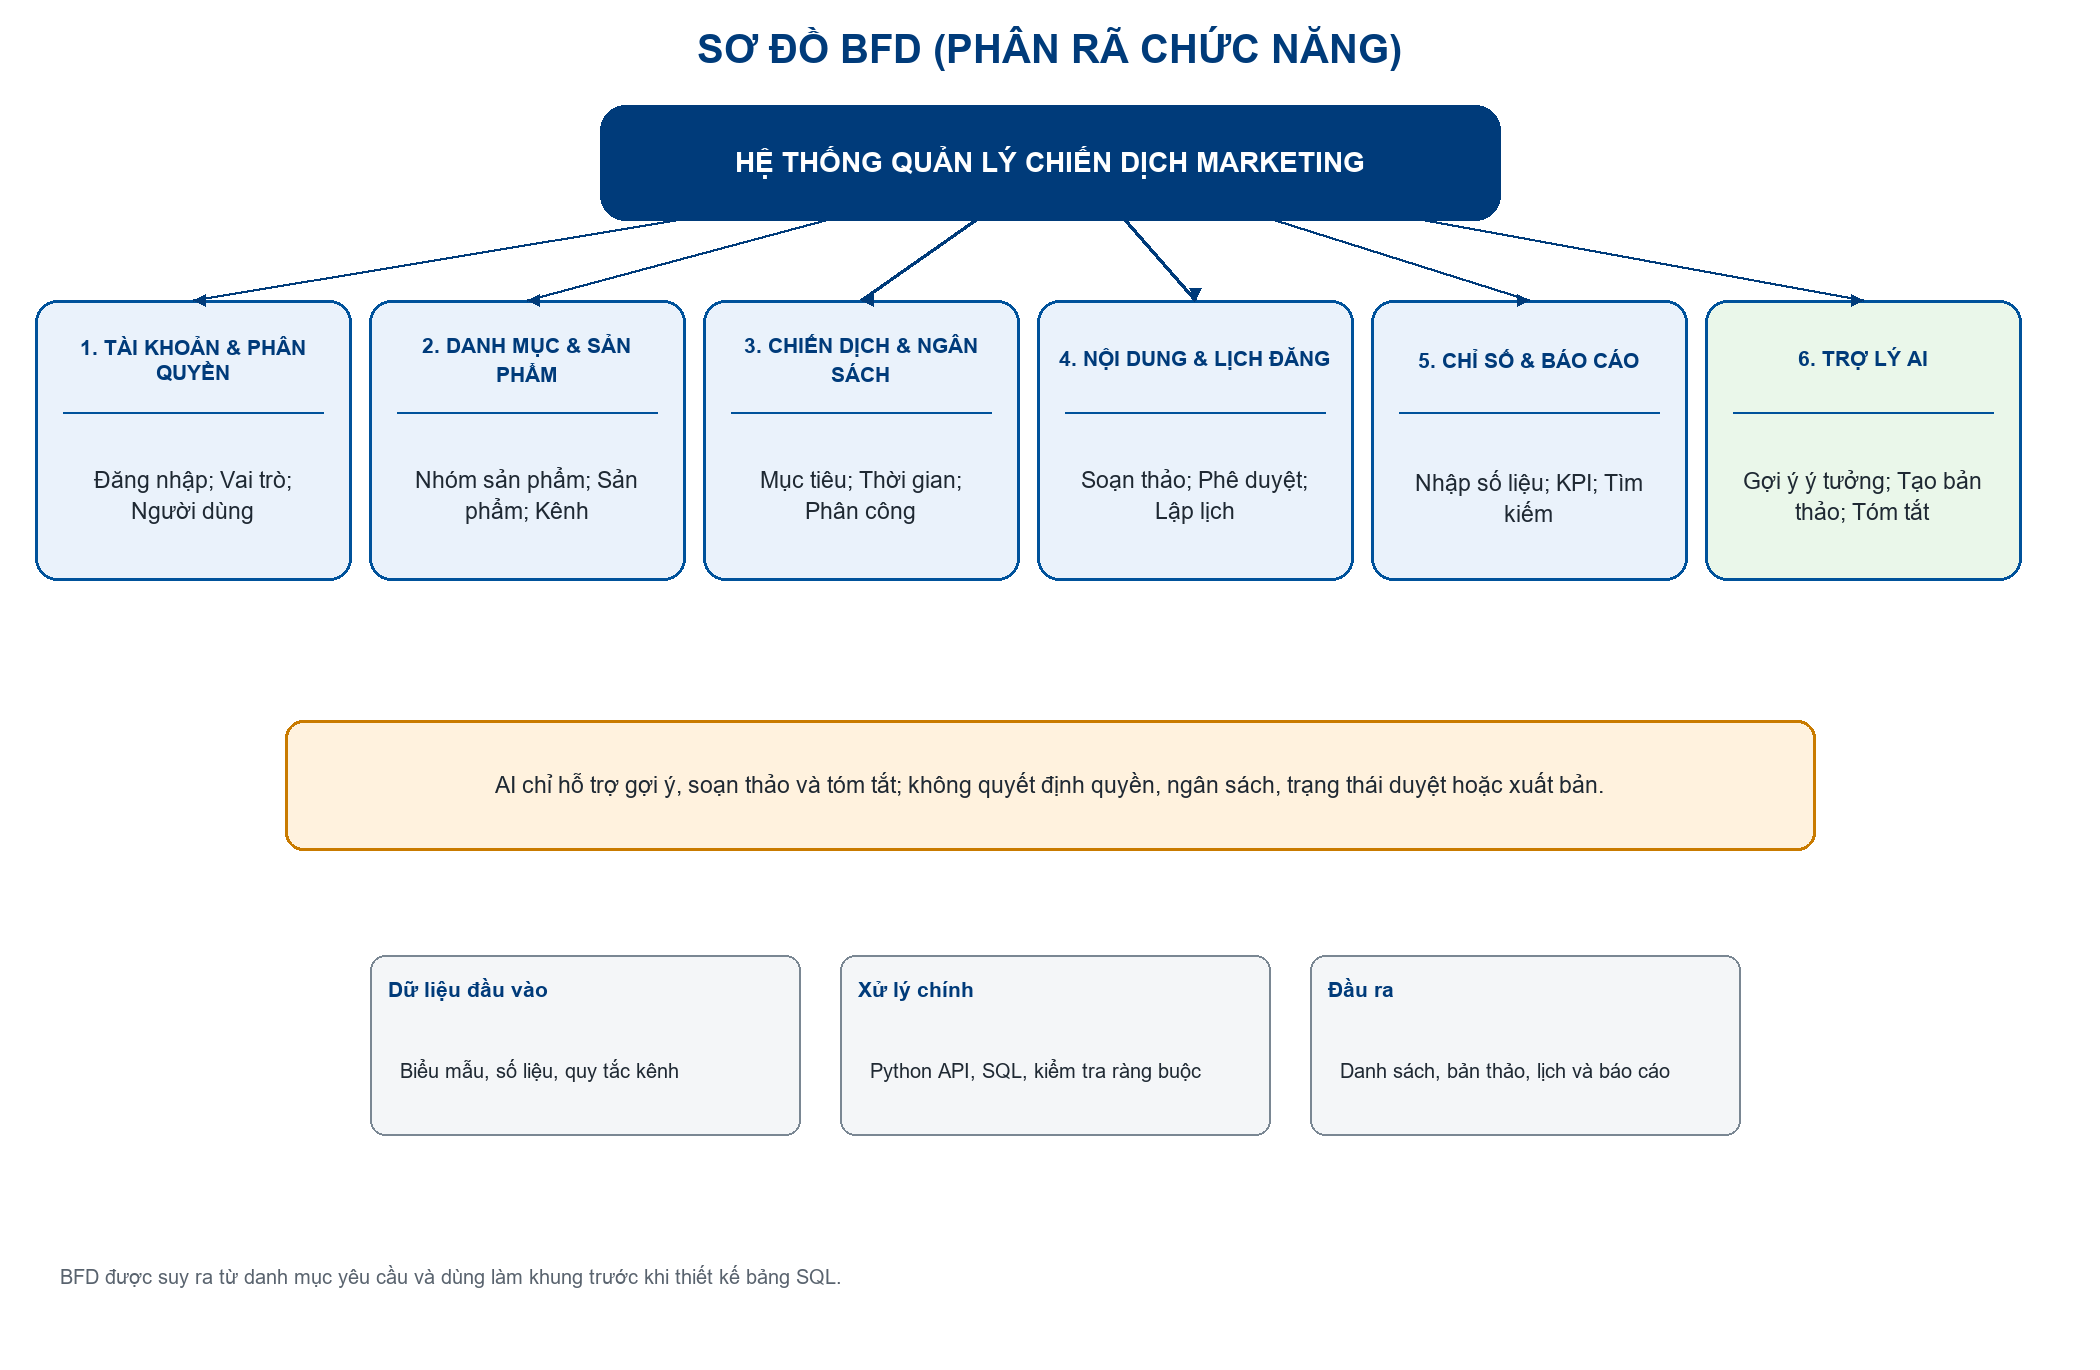
\includegraphics[width=\textwidth]{images/bfd.png}
\caption{Sơ đồ BFD phân rã chức năng hệ thống}
\end{figure}

\begin{table}[h!]
\centering
\small
\caption{Giải thích các nhánh trong sơ đồ BFD}
\begin{tabularx}{\textwidth}{|C{0.9cm}|L{4.2cm}|Y|Y|}
\hline
\textbf{Mã} & \textbf{Nhánh} & \textbf{Yêu cầu bao phủ} & \textbf{Bảng hoặc module chính}\\\hline
F1 & Tài khoản và phân quyền & P01--P03 & \texttt{users}, \texttt{auth}, \texttt{rbac}\\\hline
F2 & Danh mục và sản phẩm & P04--P06 & \texttt{product\_categories}, \texttt{products}, \texttt{marketing\_channels}\\\hline
F3 & Chiến dịch và ngân sách & P07--P09 & \texttt{campaigns}, kiểm tra ngày/tiền\\\hline
F4 & Nội dung và lịch đăng & P10--P17 & \texttt{marketing\_contents}, \texttt{marketing\_schedules}\\\hline
F5 & Chỉ số và báo cáo & P18--P22 & \texttt{campaign\_metrics}, KPI, truy vấn\\\hline
F6 & Trợ lý AI và nhật ký & P25--P26 & \texttt{ai\_logs}, \texttt{ai\_service.py}\\\hline
\end{tabularx}
\end{table}

\section{Nguyên tắc thiết kế CSDL}

\begin{enumerate}
  \item Mỗi thực thể chính có một bảng riêng và một khóa chính.
  \item Quan hệ giữa các thực thể được biểu diễn bằng khóa ngoại, không lưu tên bảng khác trong một chuỗi tùy ý.
  \item Trường bắt buộc dùng \texttt{NOT NULL}; email và tên phù hợp dùng \texttt{UNIQUE}; số tiền và số đếm dùng \texttt{CHECK} không âm.
  \item Trạng thái dùng tập giá trị rõ ràng để Python và SQL kiểm tra được.
  \item Chỉ số được lưu theo chiến dịch, kênh và ngày để có thể truy vấn, tổng hợp và tính KPI.
  \item Context đưa cho AI được lấy từ các bản ghi đã chọn; \texttt{ai\_logs} lưu nguồn và kết quả để truy vết.
\end{enumerate}

\section{Bảng SQL nhóm sản phẩm và sản phẩm}

Đây là phần SQL cốt lõi theo hướng dẫn của giảng viên. Các thuộc tính được chọn từ yêu cầu marketing: sản phẩm phải thuộc một nhóm, có giá, USP và đối tượng khách hàng. Hình dưới đây trình bày trực tiếp cấu trúc bảng, kiểu dữ liệu, khóa và ràng buộc để người đọc kiểm tra được mô hình mà không phải đọc một khối mã.

\begin{figure}[h!]
\centering
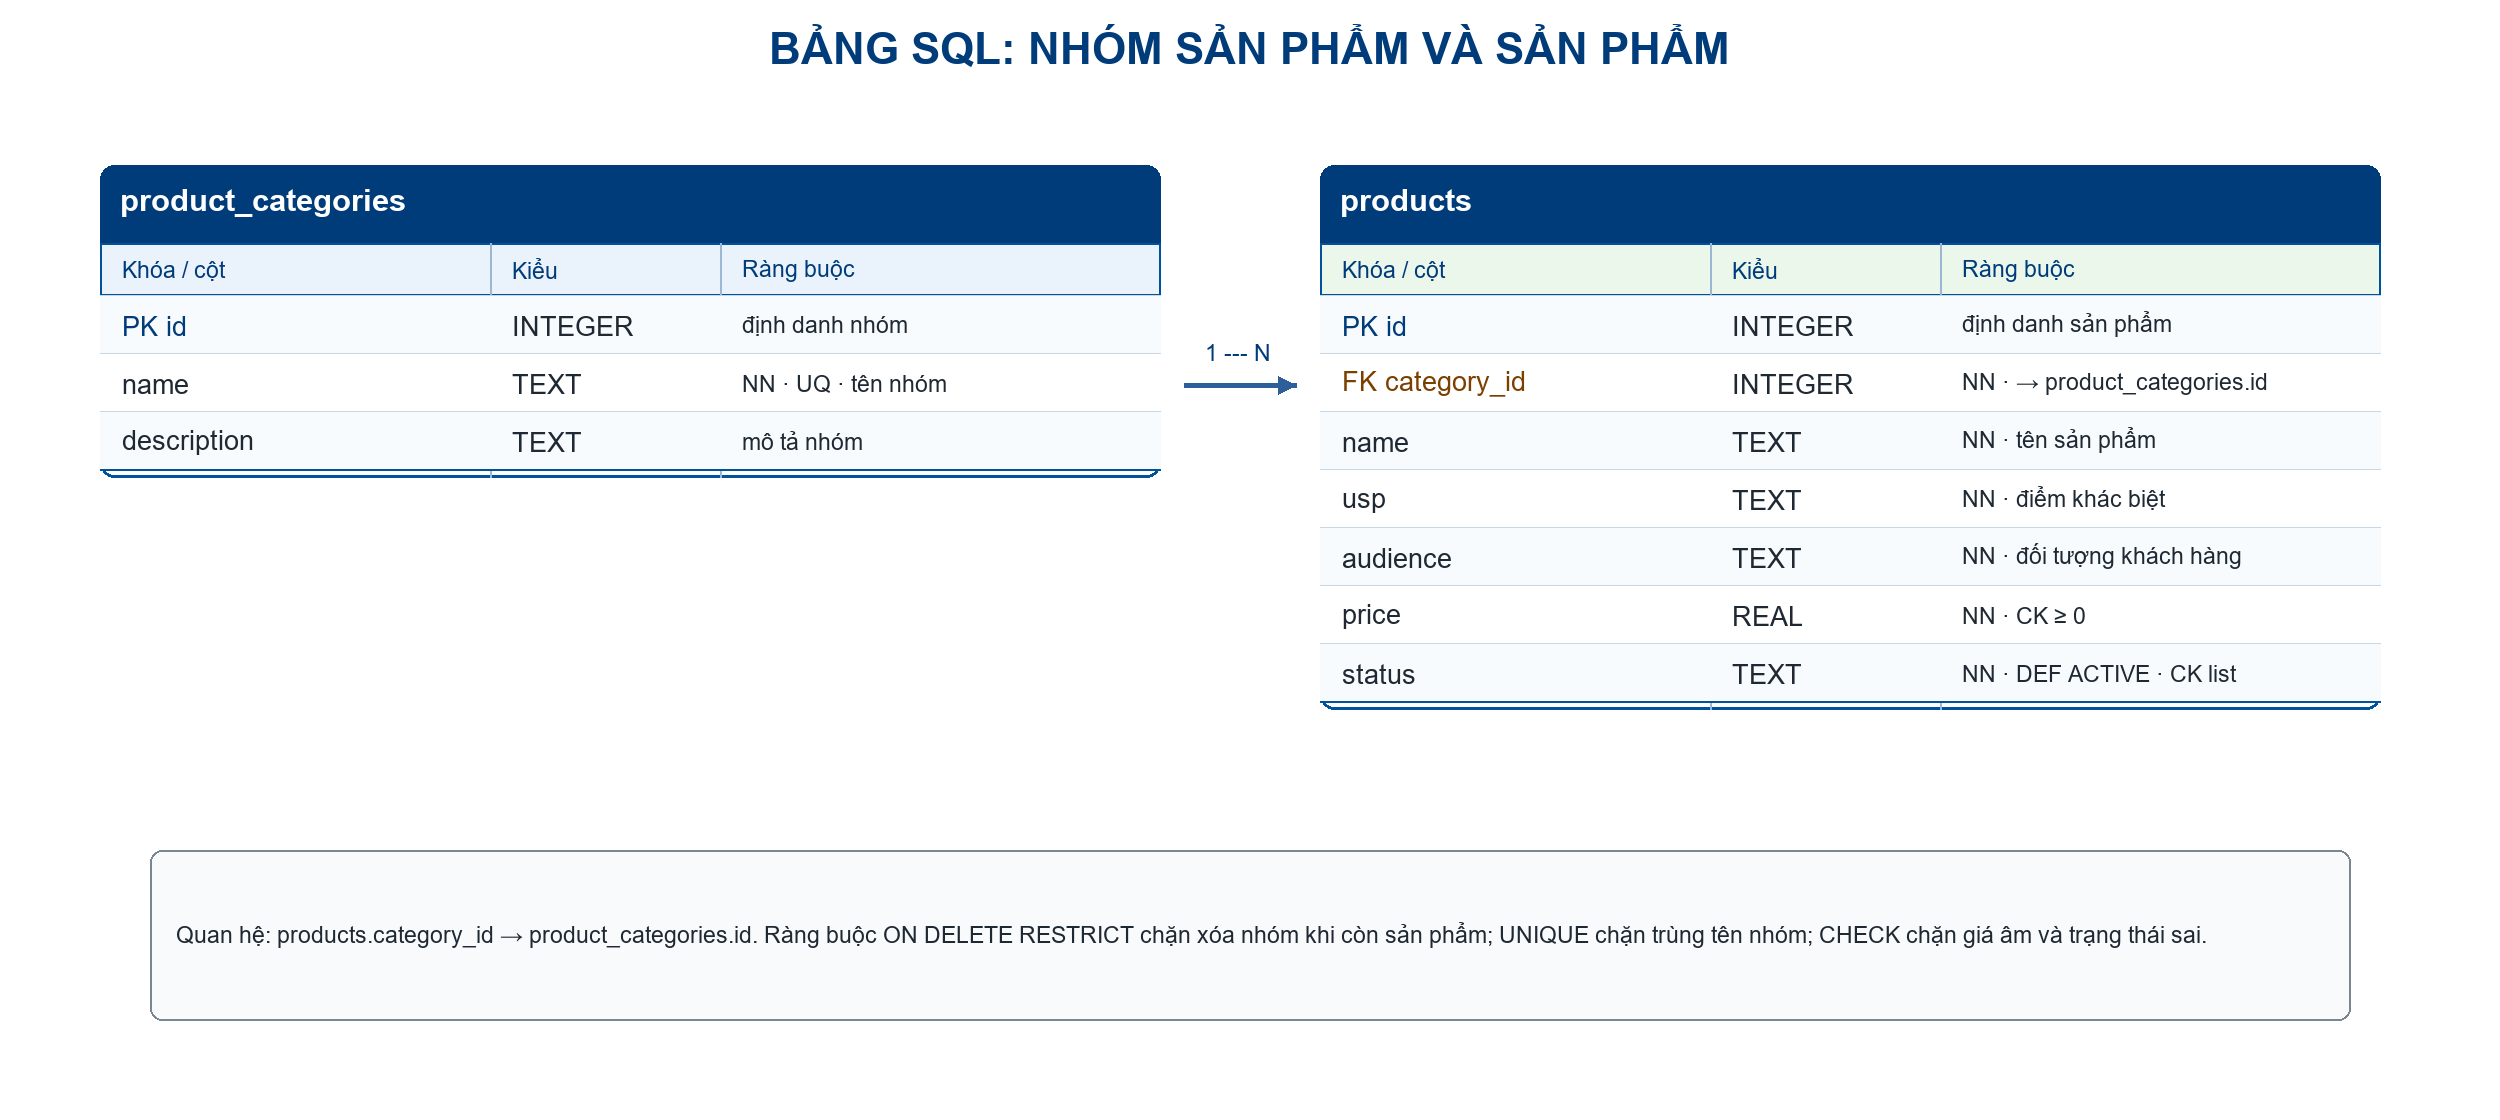
\includegraphics[width=\textwidth]{images/sql_product_tables.png}
\caption{Bảng SQL nhóm sản phẩm và sản phẩm}
\end{figure}

\noindent\textbf{Giải thích:} \texttt{products.category\_id} là khóa ngoại trỏ tới \texttt{product\_categories.id}. Vì dùng \texttt{ON DELETE RESTRICT}, không thể xóa nhóm khi vẫn còn sản phẩm tham chiếu. \texttt{UNIQUE} tránh trùng tên nhóm; \texttt{CHECK} không cho nhận giá âm hoặc trạng thái ngoài danh sách. Lệnh SQL đầy đủ tương ứng được giữ ở Phụ lục A và trong tệp \texttt{ddl.sql}.

\begin{table}[h!]
\centering
\small
\caption{Ý nghĩa các thành phần SQL trong thiết kế bảng}
\begin{tabularx}{\textwidth}{|L{3.4cm}|Y|Y|}
\hline
\textbf{Thành phần} & \textbf{Vai trò} & \textbf{Áp dụng trong hệ thống}\\\hline
\texttt{CREATE TABLE} & Khai báo một bảng và các cột dữ liệu. & Tạo \texttt{products}, \texttt{campaigns} và các bảng nghiệp vụ.\\\hline
\texttt{PRIMARY KEY} & Định danh duy nhất từng dòng. & Trường \texttt{id} giúp sửa, xóa và liên kết đúng bản ghi.\\\hline
\texttt{FOREIGN KEY ... REFERENCES} & Tạo quan hệ tới bảng cha và ngăn dữ liệu mồ côi. & \texttt{products.category\_id} phải trỏ tới nhóm có thật.\\\hline
\texttt{NOT NULL} & Bắt buộc trường phải có giá trị. & Tên, mục tiêu, ngày và các số liệu cốt lõi không được bỏ trống.\\\hline
\texttt{UNIQUE} & Không cho phép dữ liệu trùng trong phạm vi khai báo. & Email, tên nhóm/kênh và bộ khóa ngày đo không bị lặp.\\\hline
\texttt{CHECK} & Chặn giá trị không hợp lệ theo điều kiện. & Giá, ngân sách, chỉ số không âm; trạng thái chỉ nhận tập cho phép.\\\hline
\texttt{DEFAULT} & Điền giá trị mặc định khi người dùng không truyền vào. & Trạng thái mới, số liệu 0 và thời điểm tạo được thiết lập nhất quán.\\\hline
\texttt{JOIN/GROUP BY/CASE} & Nối bảng, tổng hợp và xử lý điều kiện trong truy vấn. & Lập danh sách chiến dịch và tính KPI mà không chia cho 0.\\\hline
\end{tabularx}
\end{table}

\section{Các bảng nghiệp vụ còn lại}

Các bảng còn lại được trình bày theo cùng một quy tắc. Mỗi thẻ bảng có đủ tên cột, kiểu dữ liệu, khóa chính (PK), khóa ngoại (FK), giá trị mặc định và ràng buộc kiểm tra. Tách bảng theo nhóm giúp sơ đồ đọc được trên khổ A4 và vẫn đối chiếu được với toàn bộ DDL.

\begin{figure}[h!]
\centering
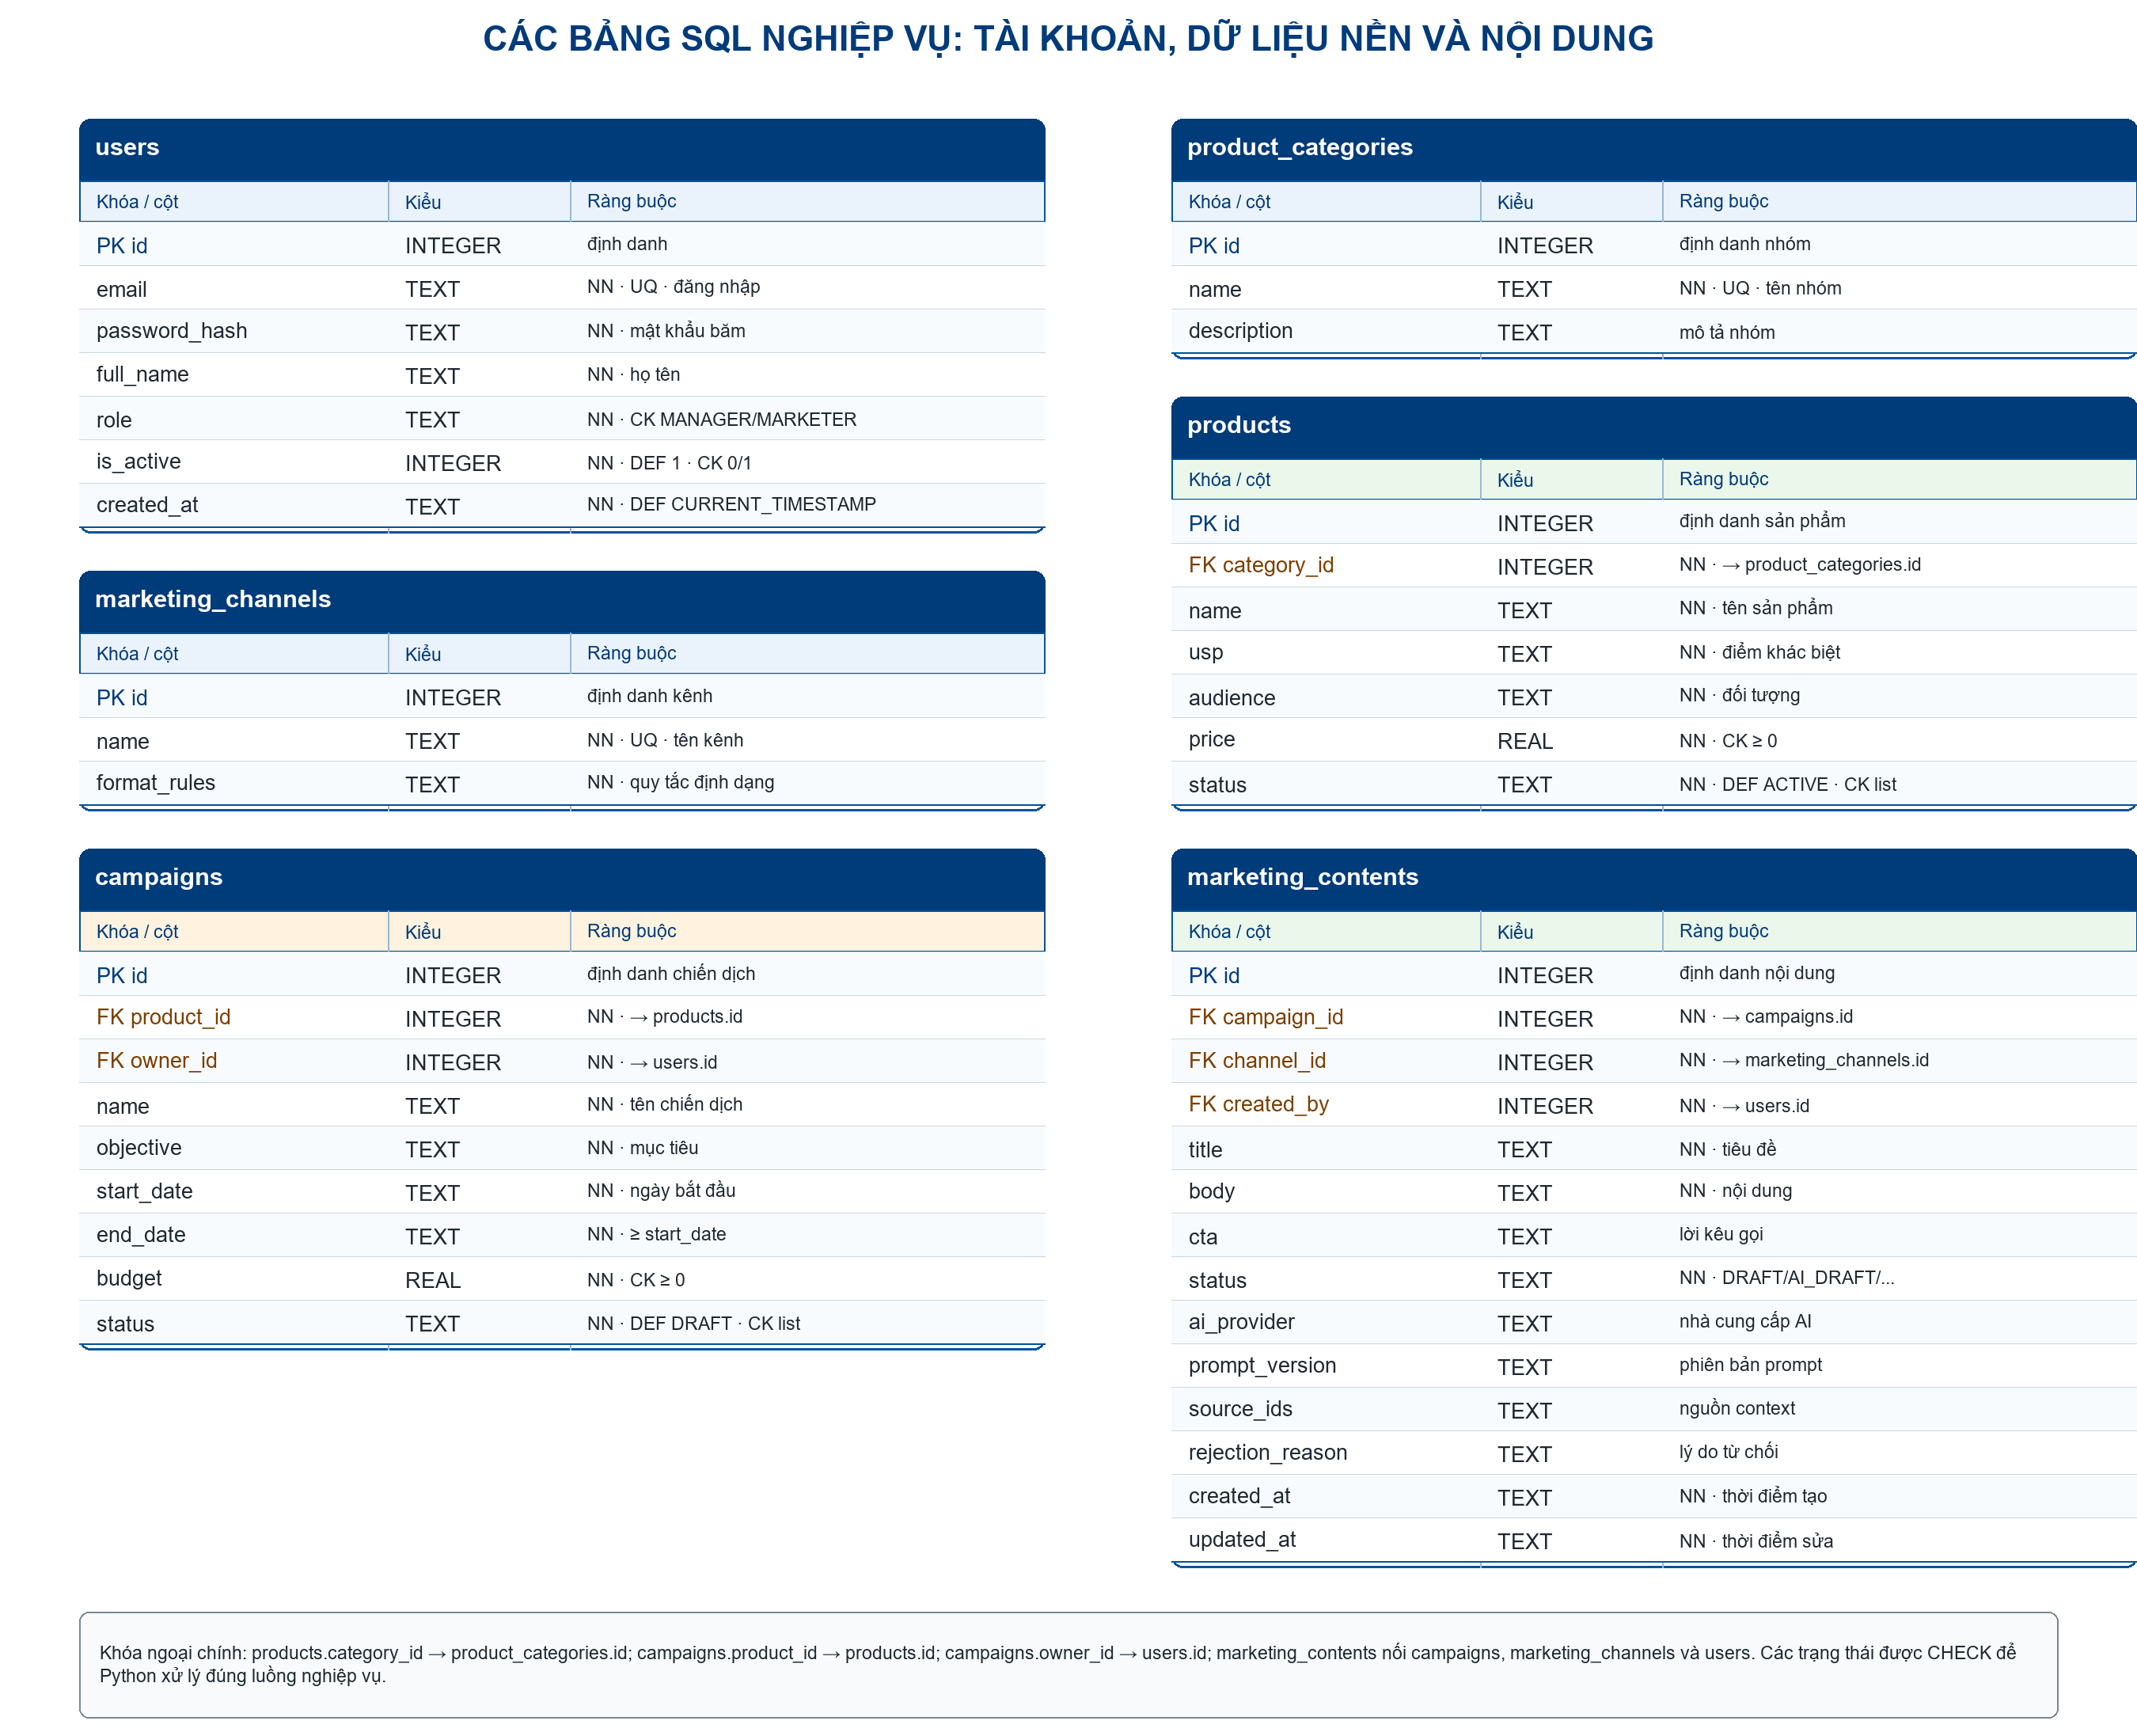
\includegraphics[width=\textwidth]{images/sql_schema_core.png}
\caption{Bảng SQL của tài khoản, dữ liệu nền, chiến dịch và nội dung}
\end{figure}

\begin{figure}[h!]
\centering
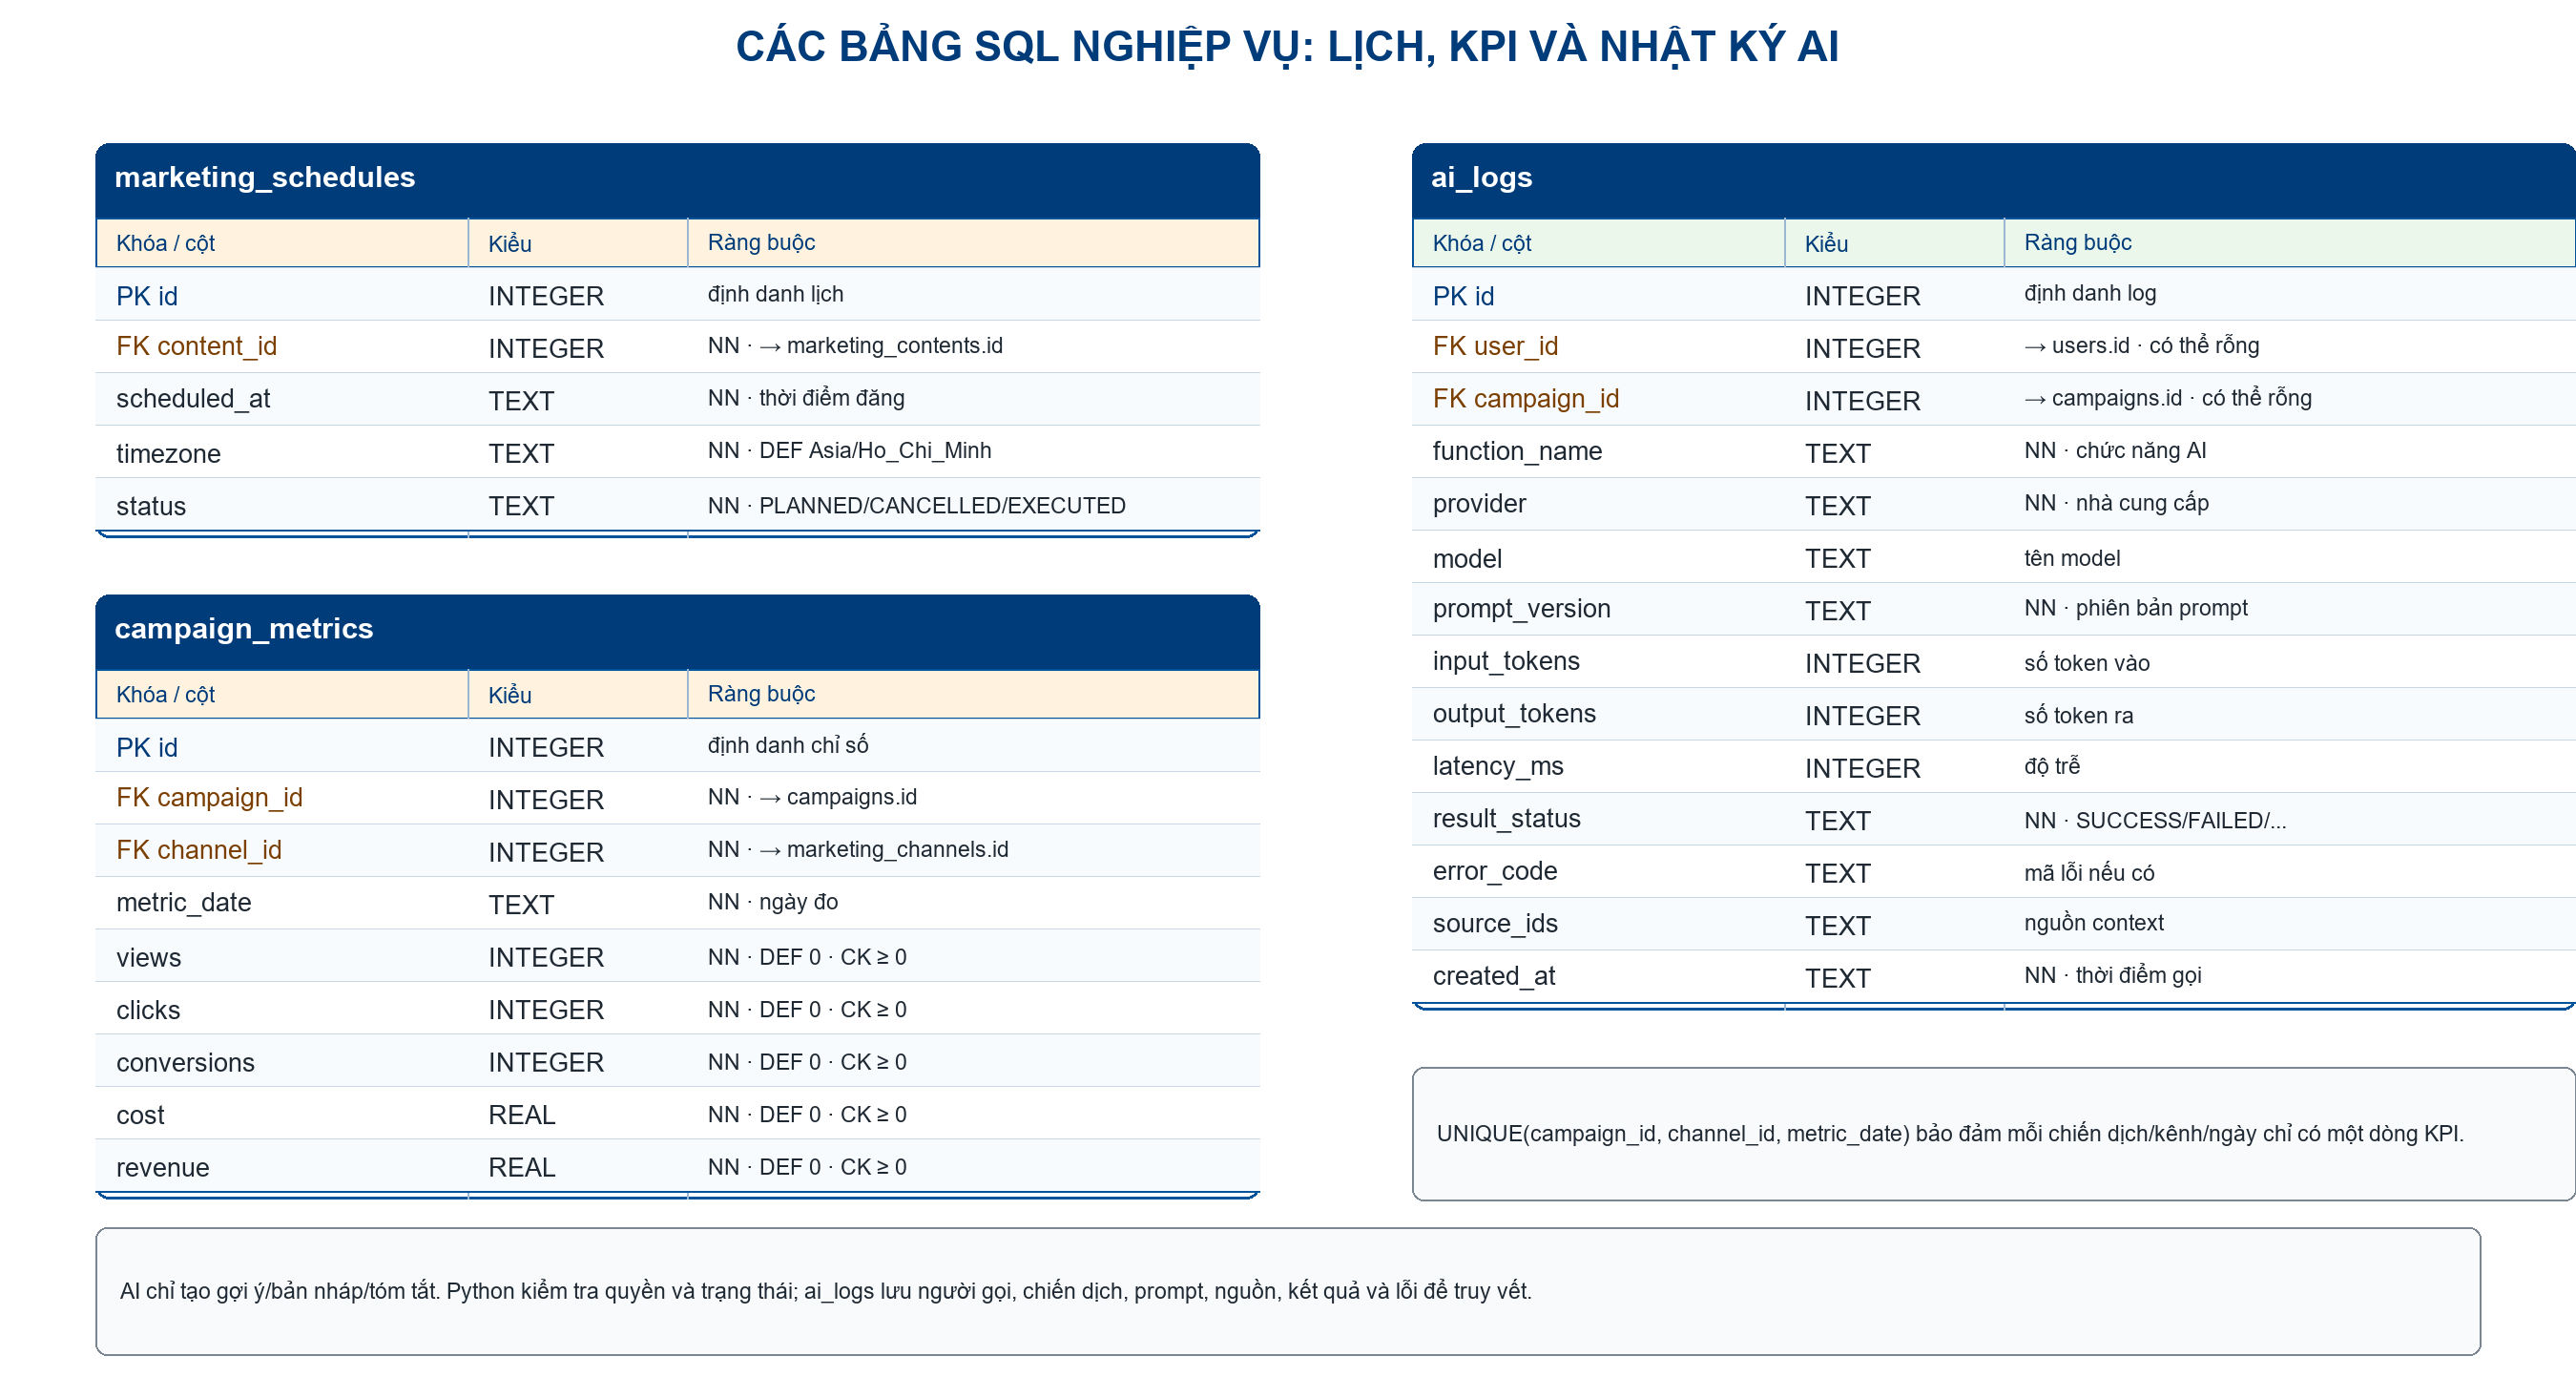
\includegraphics[width=\textwidth]{images/sql_schema_ops.png}
\caption{Bảng SQL của lịch đăng, KPI và nhật ký AI}
\end{figure}

\noindent\textbf{Từ điển dữ liệu:} cột ``Ràng buộc'' trong các thẻ bảng đồng thời ghi khóa, trường bắt buộc, giá trị mặc định, tập trạng thái và quan hệ tới bảng cha. Nhờ đó từng thuộc tính được kiểm tra ngay trên hình; DDL đầy đủ vẫn được đối chiếu ở Phụ lục A và tệp \texttt{ddl.sql}.

\section{Sơ đồ ERD suy ra từ SQL}

ERD dưới đây được vẽ sau khi xác định bảng và khóa trong DDL. Mỗi đường nối phải kiểm tra được bằng một \texttt{FOREIGN KEY}; vì vậy ERD là cách đọc trực quan của SQL, không phải một hình trang trí độc lập.

\begin{figure}[h!]
\centering
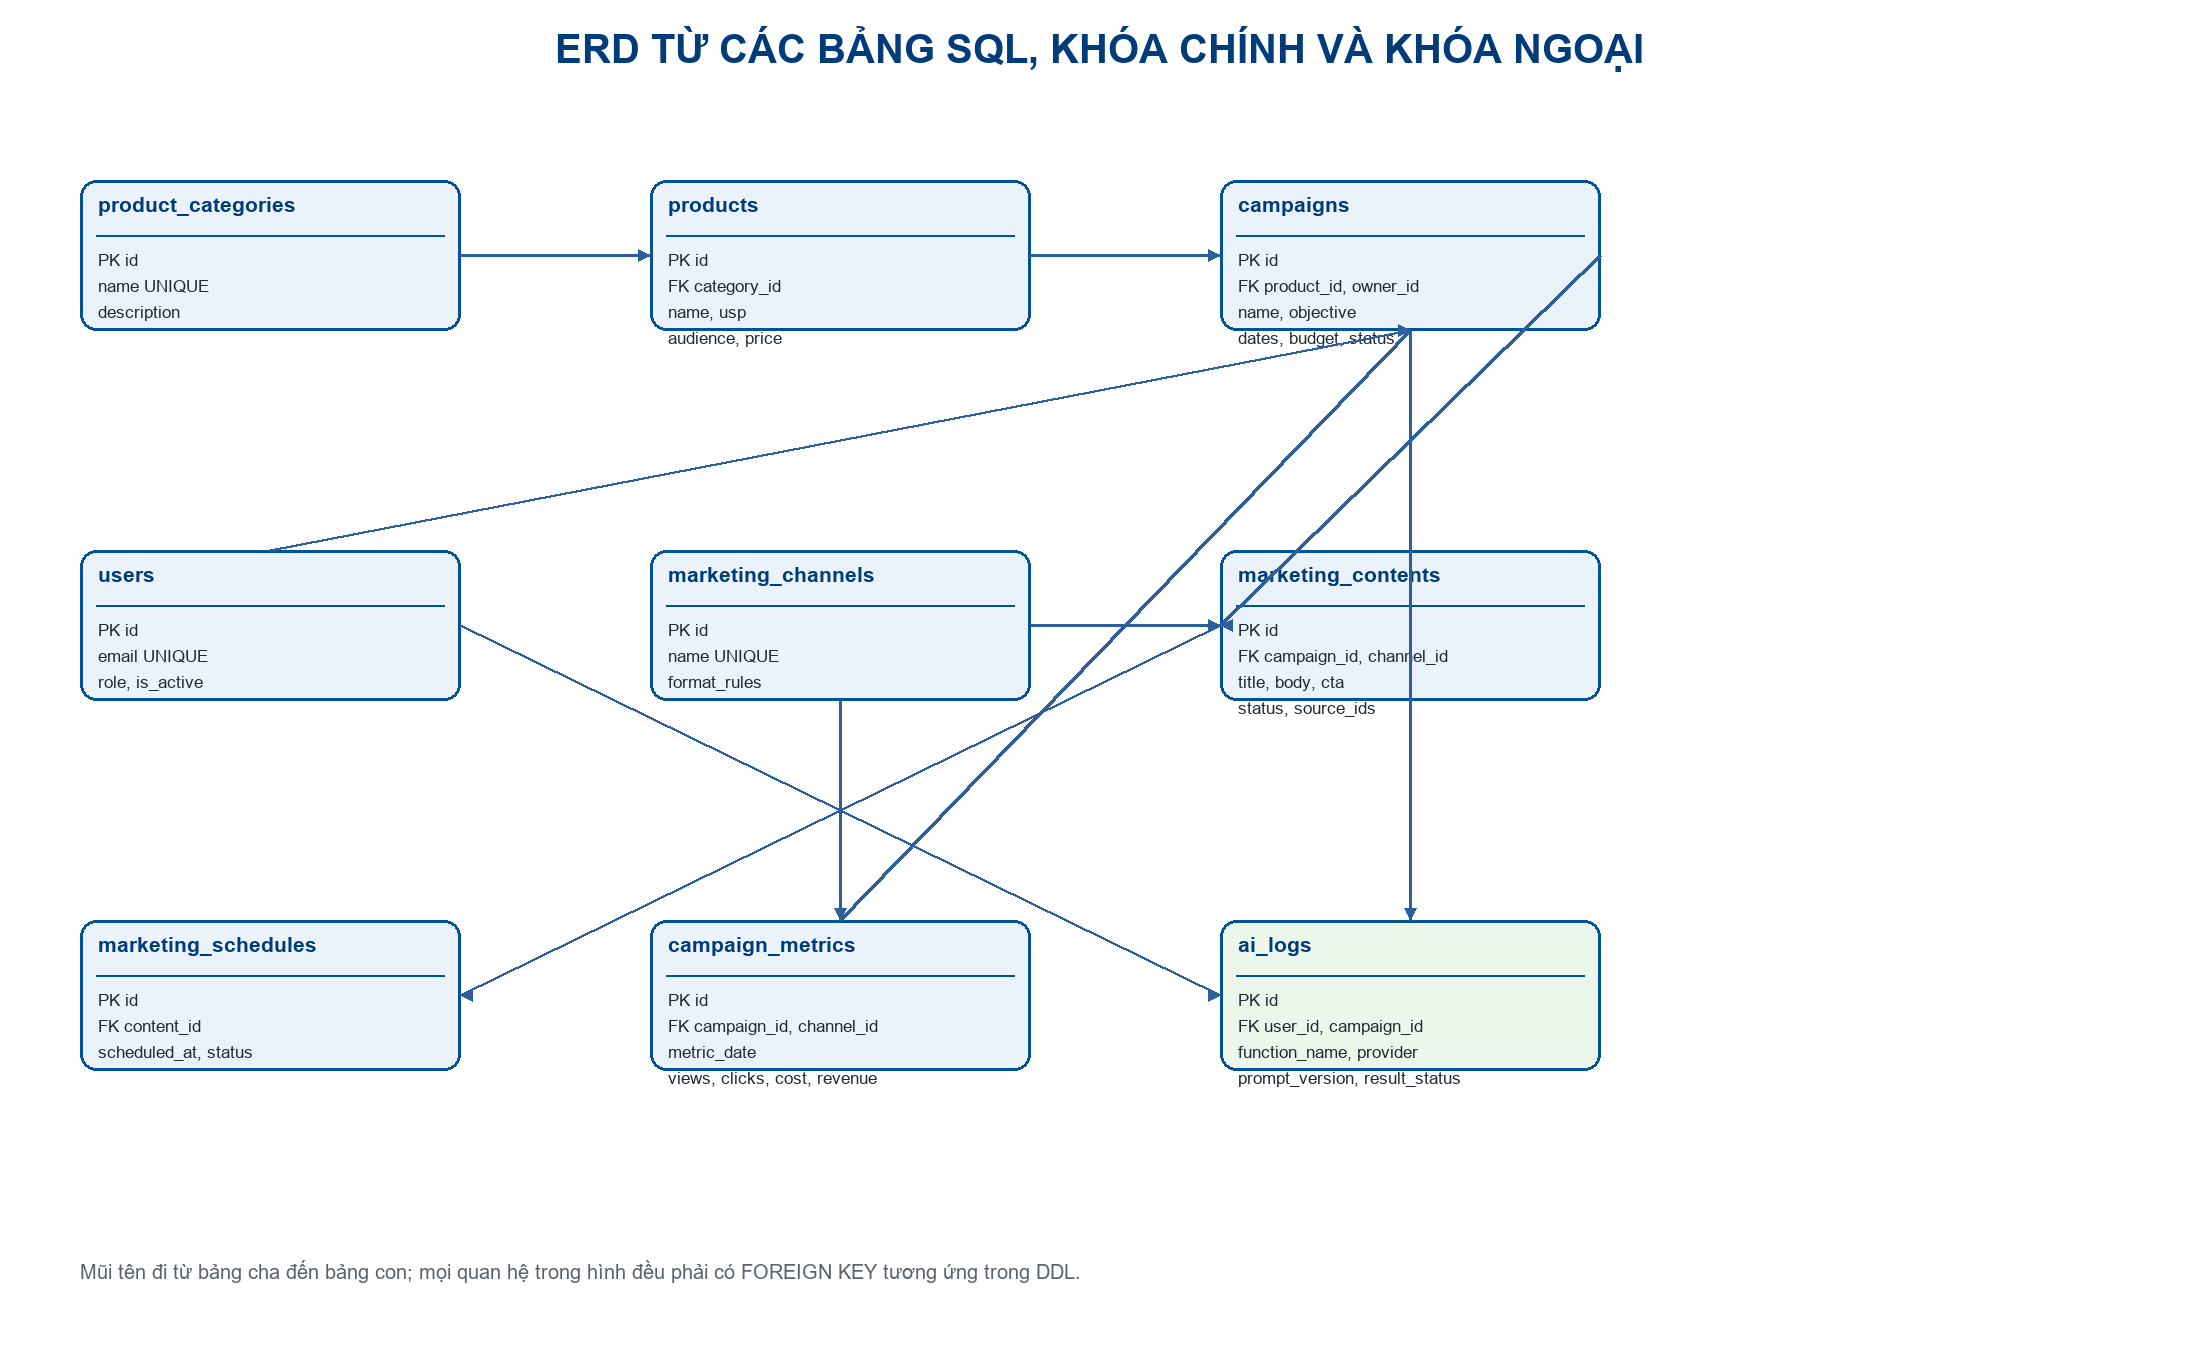
\includegraphics[width=\textwidth]{images/erd.png}
\caption{ERD từ các bảng SQL, khóa chính và khóa ngoại}
\end{figure}

\section{Các truy vấn SQL phục vụ nghiệp vụ}

\subsection{Truy vấn danh sách chiến dịch}
\begin{lstlisting}[language=SQL,caption={JOIN sản phẩm, nhóm và người phụ trách}]
SELECT c.id, c.name AS campaign_name,
       p.name AS product_name,
       pc.name AS category_name,
       u.full_name AS owner_name,
       c.status, c.budget
FROM campaigns AS c
JOIN products AS p ON p.id = c.product_id
JOIN product_categories AS pc ON pc.id = p.category_id
JOIN users AS u ON u.id = c.owner_id
WHERE c.status = :status
ORDER BY c.start_date DESC
LIMIT :limit OFFSET :offset;
\end{lstlisting}

\subsection{Truy vấn tính KPI}

\begin{lstlisting}[language=SQL,caption={Tổng hợp KPI có xử lý mẫu số bằng 0}]
SELECT ch.name AS channel_name,
       SUM(m.views) AS views,
       SUM(m.clicks) AS clicks,
       SUM(m.conversions) AS conversions,
       SUM(m.cost) AS cost,
       SUM(m.revenue) AS revenue,
       CASE WHEN SUM(m.views) = 0 THEN NULL
            ELSE 100.0 * SUM(m.clicks) / SUM(m.views) END AS ctr,
       CASE WHEN SUM(m.cost) = 0 THEN NULL
            ELSE 100.0 * (SUM(m.revenue)-SUM(m.cost))
                       / SUM(m.cost) END AS roi
FROM campaign_metrics AS m
JOIN marketing_channels AS ch ON ch.id = m.channel_id
WHERE m.campaign_id = :campaign_id
GROUP BY ch.id, ch.name
ORDER BY revenue DESC;
\end{lstlisting}

\section{Kiểm tra tính nhất quán}

\begin{table}[h!]
\centering
\small
\caption{Các điểm kiểm tra trước khi chuyển SQL thành Python}
\begin{tabularx}{\textwidth}{|L{3.0cm}|Y|Y|}
\hline
\textbf{Điểm kiểm tra} & \textbf{Quy tắc} & \textbf{Cách chứng minh}\\\hline
Khóa chính & Mỗi bảng có PK định danh bản ghi. & Đọc DDL và thử INSERT thiếu khóa.\\\hline
Khóa ngoại & Sản phẩm thuộc nhóm; chiến dịch thuộc sản phẩm/người phụ trách; nội dung thuộc chiến dịch/kênh. & Bật \texttt{PRAGMA foreign\_keys = ON} và thử FK sai.\\\hline
Giá trị hợp lệ & Tiền, số đếm không âm; ngày kết thúc không trước ngày bắt đầu. & Thử CHECK và kiểm tra mã lỗi.\\\hline
Không trùng số liệu & Một chiến dịch/kênh/ngày chỉ có một bản ghi metrics. & Kiểm tra UNIQUE.\\\hline
Trạng thái & Nội dung chỉ đi theo DRAFT, AI\_DRAFT, PENDING, APPROVED, REJECTED, PUBLISHED. & Kiểm tra CHECK và service chuyển trạng thái.\\\hline
\end{tabularx}
\end{table}

\section{Kết luận chương}

Phần này đã chuyển toàn bộ yêu cầu khảo sát thành BFD, bảng dữ liệu, lệnh SQL, ERD và truy vấn báo cáo. Hai bảng nhóm sản phẩm và sản phẩm được tạo bằng SQL rõ ràng; các bảng còn lại mở rộng đúng theo quan hệ nghiệp vụ. Chương 3 tiếp tục dùng DDL này làm nền để xây dựng hệ thống bằng Python.
